\chapter{Testing application}

Before we can run the Kubernetes cluster at Seznam.cz and start updating all applications for it, it has to be tested so we can say it will suit our conditions. For that testing I~developed an application that’ll push it to its boundaries.

The hardest task of a programmer is naming things \cite{programming-naming} but in this case my team leader came with an idea -- the Tarsier. Tarsiers are small primates with enormous eyes. Each eyeball is large as its entire brain \cite{tarsier}.  That means they will probably not invent anything new and useful, but they can watch and see everything -- which quite fits for my testing application needs. It won’t be doing anything extraordinary, it just has to test the cluster and find its weaknesses.

The basic requirements on the Tarsier are to heavy load the machine resources, to simulate high CPU and RAM usage, to simulate I/O operations (so it will have to request permissions on some persistent storage), to raise controlled faults, deadlocks and segmentation faults and finally to simulate a network communication.

Of course the Tarsier will have to log its activity and probably also expose its inner statistics and metrics.

When designing the Tarsier I~have to think about implementing new functions in the future, so it should be modular. User need to be able to control the Tarsier’s behavior from the outside, because deploying a new image just because of a different configuration to make use of another set of its skills would be slow and inefficient.

Another important thing is that one Tarsier will hardly be able to push the cluster to its boundaries, but if we employ many monkeys at once that can communicate with each other and start using the network at the same time for example, that is something that should be able to easily find the limits of the Kubernetes cluster.

\section{Designing Tarsier}

I~designed the Tarsier as a modular application. However, as there there are no dynamic libraries in Go that could be joined together during the runtime, every application with all its dependencies is built from the source. So I~created a plugin interface and a plugin registration function that will store plugin’s factory method, so Tarsier can invoke the plugin later with the desired configuration.

As the Tarsier will have to do many different tasks, I~decided to separate each task to the Command interface and plugin that has some commands will register them.

\begin{lstlisting}[language=go,caption=Tarsier plugin's interfaces]
  type Plugin interface {
  	Init(config interface{})
  }
  type HasConfigStruct interface {
  	ConfigStruct() interface{}
  }
  type HasCommands interface {
  	Commands() []Command
  }
  
  type Command interface {
  	Execute(data interface{})
  	Name() string
  	Description() string
  }
  type HasDataStruct interface {
  	DataStruct() interface{}
  }
\end{lstlisting}

For remote controlling the Tarsier I~use HTTP requests, so the Tarsier is a modular API server, where plugins can register themselves and their commands and the Tarsier then waits for orders and executes the appropriate command when invoked. Each plugin can claim self-specific configuration and each command may demand specific data. There can also be plugins with no commands because it is possible that in the future the requirements on the Tarsier might change.

At the moment Tarsier starts as a HTTP server with one handler on the 
\lstinline{/exec} URL and it accepts YAML POST requests (and because valid JSON data comply with the YAML specification, it accepts JSON POST requests as well). The structure of the body is the following:
\pagebreak
\begin{lstlisting}[language=yaml,caption=Command 'spin\_cpu' body structure]
command: "heavy_load/spin_cpu"
data:
    duration: "15s"
wave: 
    remain: 3
    buddies: 10
\end{lstlisting}


If the command named \lstinline{heavy_load/spin_cpu} is registered and if it implements the HasDataStruct interface, the data from the body will be unpacked to the DataStruct method returned value and the command will be executed with that structure. This will happen in a separate goroutine so the handler can also process the wave part. The wave remain is a number of how many waves are remaining to do. If it is greater than zero that means this Tarsier will have to send this request beyond and notify 10 its buddies with the same data as he gets. Obviously the wave remain value will decrease.

The waves are spread exponentially and it is possible that some request will come back to the same Tarsier that sent them but that does not matter because I~want to test the cluster and some random behavior is even welcome. Let’s see another example command:
 
\begin{lstlisting}[language=yaml,caption=Command 'write' body structure]
command: "persistent_storage/write"
data:
    amount: "100 MB"
    files: 10
wave: 
    remains: 3
    buddies: 3
\end{lstlisting}
 
This will start writing 100 MB into 10 files in parallel on each Tarsier. And also this command will be sent to 3 more Tarsiers randomly chosen from friends list. The flow of the wave with 9 tarsiers might look like in the following example \ref{fig:tarsier-wave}. 
                
\begin{figure}[htb]\centering
  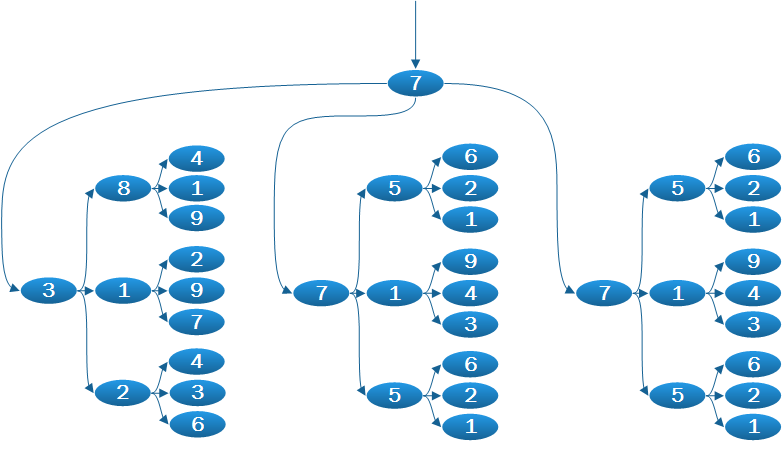
\includegraphics[width=1\textwidth]{images/wave.png}
  \caption
    [Wave propagation in Tarsier]
    {Wave propagation in Tarsier}
  \label{fig:tarsier-wave}
\end{figure}

\section{Tarsiers synchronization}
To be able to discover all the Tarsiers and to help each one of them find the others so it can send waves to them I~will use Consul \cite{consul}. Consul is designed for service discovery and makes it easy to register services and to discover them later. Each Tarsier will register itself at startup and then it will periodically check its buddies. To ensure that Consul will provide only active Tarsier instances, it has multiple types of health checks. Tarsier will have to provide some service stats.

At first I~wanted to just add some special URLs for this service stuff such as \lstinline{/health_check} and \lstinline{/metrics} but then I~realized that in the future those URLs may be needed and also those URLs don’t have to be accessible from the public network so I~designed Tarsiers with another extra interface on its own port were private data will be provided. There will be health check and metrics handler with Prometheus statistics about how many requests have been served and what commands were executed and if they were successful. I~also created a command handler where all the registered commands with their names and descriptions are provided. Because there will be plugin to simulate heavy load of memory and CPU I~add a handler that shows runtime statistics from Go. There can be seen how much memory is allocated to the Go runtime, a garbage collector statistics and much more interesting data.

\section{Tarsier plugins and their commands}

\subsection{Heavy load}
Plugin for simulating heavy load of memory and CPU
\begin{description}
  \item[Gobble RAM] will gobble as much RAM as is specified in the data. When this amount of memory is not possible to allocate it will try to resize the amount with the specified ratio and return how many bytes it finally allocated. Memory is allocated via mmap system call so the garbage collector will not free it and is filled with zeros otherwise system will not physically allocate it.
  \item[RAM stats] will show allocated mmap regions with their sizes.
  \item[Free RAM] This command will unmap allocated region. Its data is the index of the region obtained from the RAM stats command or -1 which means to free all allocated spaces.
  \item[Spin CPU] spins the CPU for the specified time. The spinning is simply done by an infinite loop with acomputation (multiply and division) with float64 numers.
\end{description}

\subsection{Faults}
\begin{description}
  \item[Deadlock] will create the specified number of goroutines that will be set to be sticky with system threads (otherwise Go runtime is allowed to move them all into single system thread, so it has no effect) and deadlock them all waiting for mutex unlock. After the defined time the handler will unlock the mutex so all goroutines will finaly end.
  \item[Segfault] will simulate segmentation fault. It uses Go unsafe package pointer to variable, which is moved out of bounds and dereferenced. The whole Tarsier will fault and it is expected that Kubernetes will start new instance.
\end{description}

\subsection{Net}
This package is here to wrap all the network commands. There are no commands for writing or reading from the network but that can be easily simulated with a dummy command to the Tarsier where waves count will be high enough.

\begin{description}
  \item[Dial] will open a new network connection to the specified address. It can open a new TCP or UDP connection and also this connection can be established directly to an IP address or to a domain name with its resolving. Those connections are set not to timeout and are not closed.
  \item[Stats] will show the network connections usage.
  \item[Close] will close the specified network connection from the Stats command. When -1 is set it closes all connections.
\end{description}

\subsection{Persistent storage}
Plugin that is working with persistent storages, typically hard disks. This plugin needs to get directory from configuration of Tarsier otherwise system temporary directory is used.

\begin{description}
  \item[Open FD] will open as many file descriptors as defined.
  \item[Read] This command will read the specified amount of bytes from defined file. Typically \lstinline{/dev/urandom} is set as a file. There is also an option how many concurrent readers are supposed to be created.
  \item[Write] will write the specified amount of bytes to opened file descriptors. There can be set how many concurrent writers are supposed to be created and each one is writing to its own file. If there is not enough file descriptors ready, new ones will be opened.
  \item[FS stats] will show usage of file descriptors, their names and sizes.
  \item[Close FD] will close the specified file descriptors from the FS stats command. When -1 is set then all file descriptors are closed and the files are deleted from the hard drive.
\end{description}

\subsection{Sleeping beauty}
Plugin for simulating requests delay.
\begin{description}
  \item[Sleep] will answer after the specified time expires.
\end{description}
